Cassandra is an open source NoSQL database designed for high availability of large amounts of data with no single point of failure. [Need citation]

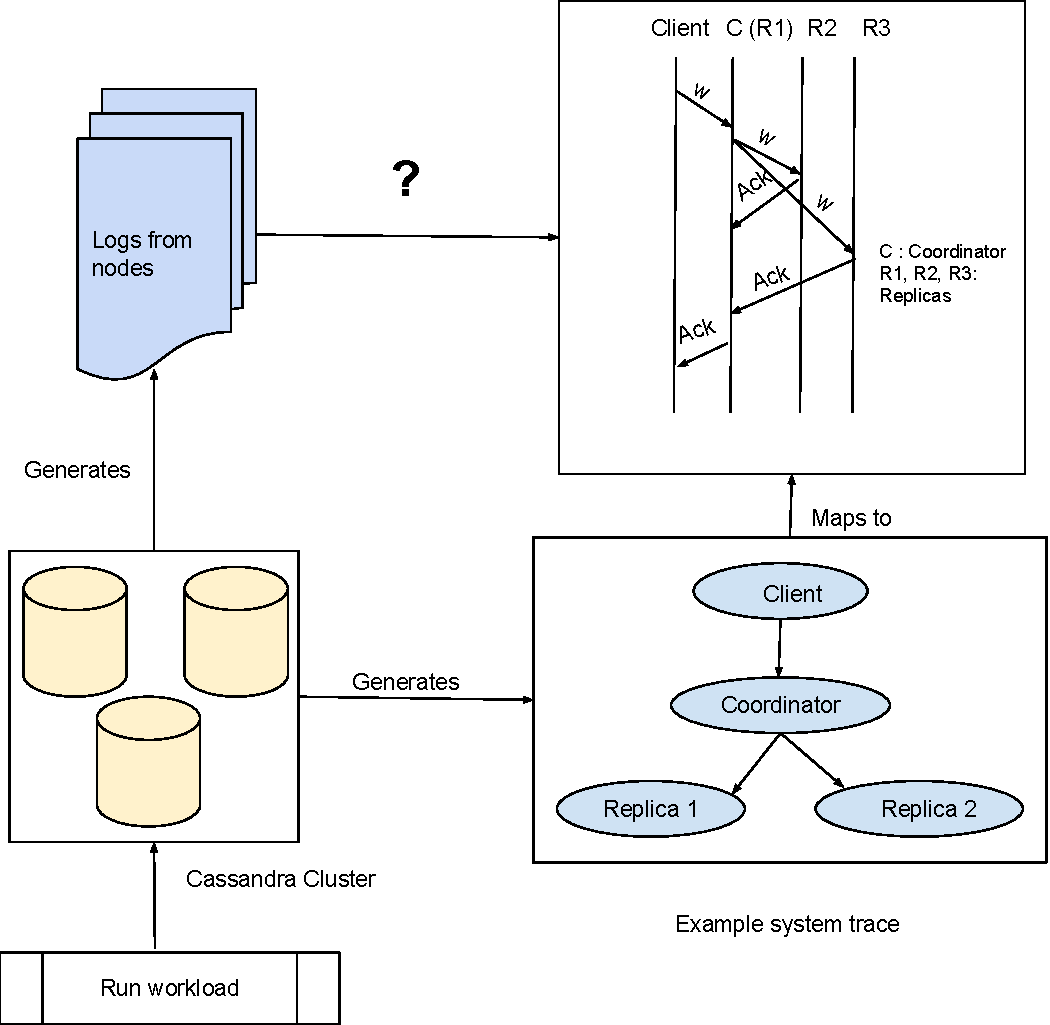
\includegraphics[scale=0.35]{figures/system_model.pdf}

Integration of Zipkin with Cassandra enables us to obtain both the system traces as well as logs from running a query against the database. [Need citation]

We run a single insert query on a replicated cluster and collect both system logs as well as Zipkin traces in JSON format. 

We map the traces obtained to a Lamport diagram of the interaction. The questions we will be addressing are:
\begin{enumerate}
\item Can we reduce the number of dependencies so we can visualize the result?
\item How closely can we approximate the actual interaction?
\end{enumerate}
